\chapter{Low fidelity prototype}

\section{Prototype}
The first of three prototypes is the lo-fi prototype, which in this project is created by hand on paper. To interact with this system, the user must see the prototype as a touchscreen, and the drawn RFID and barcode scanner is also simulated. The” wizard of oz” method is now used to navigate between pages, and when the user touches the screen or uses one of the scanners, a new piece of paper is placed on top with the new page. \\
\begin{figure}[H]
\centering
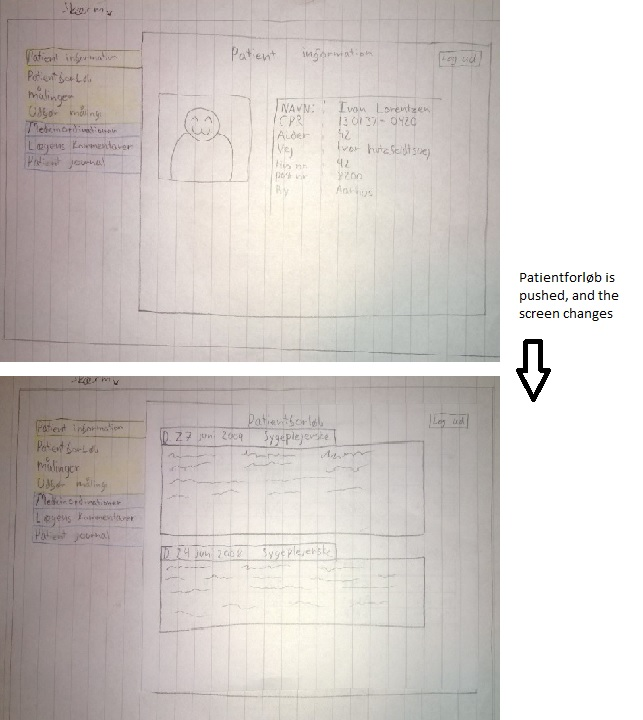
\includegraphics[width=0.75\textwidth]{billeder/lofi}
\caption{Low Fidelity Prototype}
\end{figure}
\section{Obtaining usability goals}
With the lo-fi prototype we aimed to give the user a good overview of what was available in the system by making tabs in the left side of the screen showing all options available.\\
We hoped this would ease the use of the system and it also solved another goal namely effectiveness. Since you can go everywhere in the system with one touch and from all screens.\\
\section{Obtaining user experience goals}
The goal with the lo-fi prototype was mostly to get started and get an idea of where we were heading. We tried to make it satisfying to use by making it fast and easy to work with. This also helps achieving some of the other user experience goals such as engaging, helpful and fulfilling.\\



\section{Peer review}
The peer review was used to test the main idea of the application, how easy it was to navigate in, and to get feedback on the preliminary design. A group of three people reviewed the system, by performing 4 different tasks on the Wizard of Oz lo-fi paper prototype while they were evaluated. To each task were noted the exact time and how they did on a scale from 1 to 3, with the following definition:
\begin{table}[H]
    \begin{tabular}{|p{4cm} p{10cm}|}
    \hline
    1 = Failure         & The user cannot complete the task. \\
    ~ & If the user navigates wrong more than 3 times, this counts as a failure. \\ \hline
    2 = Partly succes   & User completes the task, with a maximum of 3 wrong navigations, and within the time limit on 30 seconds.    \\ \hline
    3 = Complete succes & The user completes the task without wrong navigations and within the time limit on 20 seconds.              \\ \hline
    \end{tabular}
\end{table}

\subsection{Results from peer review}
The first metrics and statistics from the lo-fi peer review only tells that the system has a quick learnability curve, and besides this gives results to compare to the mid-fi peer review.The peer review group had at the end the chance to give overall comments, which was very useful to the development of the mid-fi prototype. 
Some of these comments included:\\
\begin{itemize}
\item Bigger buttons
\item More explanatory text
\item Results and important text on top
\end{itemize}

